%! TEX root = main.tex
\chapter{PetIBM: a Distributed-GPU Incompressible Navier-Stokes Solver}\label{chap:petibm}

PetIBM is a C++ library that helps create new incompressible flow solvers for large-scale and distributed GPU computing.
The core design philosophy of PetIBM is to allow the easy creation of a solver that fits into Perot's framework \cite{perot_analysis_1993} for projection methods.
Combining Perot's framework and staggered grids, PetIBM does not need pressure boundary conditions.
Pressure boundary conditions have caused many headaches for CFD practitioners \cite{gresho_pressure_1987,sani_resume_1994}.

On top of the vanilla projection method from Perot, the primary use case of PetIBM is to create solvers of the immersed-boundary projection method (IBPM \cite{taira_immersed_2007}) and its derived works.
With PetIBM, users focus their time on defining components and algorithms in Perot's framework and leave the parallelization to PetIBM.
Solvers created with the PetIBM library run on distributed-memory architectures, including GPU clusters.

To our knowledge, another work similar to PetIBM is IBAMR \cite{griffith_adaptive_2007,bhalla_unified_2013}. 
PetIBM and IBAMR use different immersed-boundary schemes.
IBAMR is based on Peskin's immersed-boundary formulation \cite{Peskin2002} and implements adaptive mesh refinement.
However, IBAMR does not have GPU capability, as far as we know.

Though PetIBM's primary role is a library, it includes several flow solvers for different flow applications and solving schemes.
These solvers serve as examples for users to learn how to create their own.
We also use these solvers to conduct studies in fluid dynamics (e.g., \cite{mesnard_reproducible_2017}).
All baseline data in the PINNs' benchmarks in chapter \ref{chap:pinn-cases} were generated by a decoupled IBPM (decoupled immersed-boundary projection method \cite{li_efficient_2016}) shipped with PetIBM.
In the remaining dissertation, PetIBM often refers to this decoupled IBPM solver rather than the library itself.

The following section briefly introduces the decoupled IBPM.
Section \ref{sec:petibm-impl} describes the higher-level software design of the PetIBM library and the solver.
The decoupled IBPM solver will be used to generate baseline data for benchmarking PINNs, so verification, validation, and performance benchmarks are done and shown in sections \ref{sec:petibm-vv} and \ref{sec:petibm-perf}.

For interested readers, a complete PetIBM installation also includes a basic Navier-Stokes equation solver (for flows without objects), the original IBPM solver, and a solver for moving bodies with prescribed motions.
These solvers, however, are out of this work's scope.
Their descriptions can be found in the documentation of reference \cite{chuang_petibm:_2018}.

\section{Decoupled Immersed-Boundary Projection Method}\label{sec:petibm-math}
%! TEX root = main.tex

Immersed-boundary methods solve fluid flow problems with the presence of solids by adding a body-force term to the Navier-Stokes equations.
This body-force term mimics the interface between fluid and solids.
Depending on the chosen formulations and schemes, the solids may be either rigid or deformable.
They can be stationary objects, objects moving under prescribed motions, or objects moving under feedback forces from fluid.
Different immersed-boundary methods may use different formulations for this body-force term to model the fluid-solid interfaces.

To be more precise, this forcing term models the force applied to the fluid by solids.
As this forcing term is part of the fluid governing equations defined in Eulerian coordinate systems, it is resolved on the same computational grid of the fluid, and solid-fluid interfaces are not anymore boundaries of the fluid's computational domain.
In other words, body-fitting meshes are unnecessary.
A benefit of such an approach is that a structured grid can be applied to solve flow problems with the presence of an object with complex geometry.

Consider a fluid problem with a fluid-solid interface.
$\Omega$ and $\Gamma$ corresponding to the whole domain of our interest and the fluid-solid interface.
The fluid-solid interface may be moving when viewing from a fixed coordinate system.
Given a time $t$ and a spatial coordinate $\vec{x}$ in an Eulerian coordinate system defined in $\Omega$, we can write the following Navier-Stokes equations for incompressible flow and the immersed-boundary projection method (IBPM):
\begin{subequations}\label{eq:mod-ns}
    \begin{align}[left=\empheqlbrace\,]
        &\pdiff{\vec{u}}{t} + \left(\vec{u} \cdot \nabla\right) \vec{u}
            =
            -\frac{1}{\rho}\nabla p + \frac{1}{Re} \nabla^2 \vec{u} + 
            \int\limits_{\Gamma} \vec{f}\left(\vec{\xi}\left(s, t \right), t\right) \delta\left(\vec{\xi}\left(s, t\right)-\vec{x}\right)\diff {\Gamma} 
            \label{eq:mod-ns-momentum} \\
        &\nabla \cdot \vec{u} = 0 \label{eq:mod-ns-cont}\\
        &\int\limits_{\Omega} \vec{u}\left(\vec{x}, t\right) \delta \left(\vec{x}-\vec{\xi}\left(s, t\right)\right)\diff\Omega
            =
            \vec{u}_{\Gamma}\left(s, t\right)
            \label{eq:mod-ns-body-vel}
    \end{align}
\end{subequations}

$\vec{u}$, $p$, $Re$, and $\rho$ are the velocity vector, pressure, Reynolds number, and fluid density, respectively.
$\vec{u}$ and $p$ are functions of $\vec{x}$ and $t$.
Though $\rho$ and viscosity can also be functions of $\vec{x}$ and $t$ for incompressible flow, we simply treat them as a constant in this work.
$s$ denotes the coordinate in a Lagrangian coordinate system defined on $\Gamma$.
For example, such a Lagrangian coordinate system is a curve in 2D problems, and a single scalar $s$ is enough to represent a coordinate on the interface.
$\vec{\xi}(s, t)$ is the coordinate in the Eulerian coordinate system that correspond to a Lagrangian coordinate $s$ on $\Gamma$ and at time $t$.
$\vec{u}_\Gamma$ represents the velocity of the fluid-solid interface.
Note $\vec{u}_\Gamma$ is a concept from the viewpoint of Lagrangian coordinate system.
$\vec{f}$ is the vector of force applied on fluid due to the presence of the fluid-solid interface.
It is defined in $\Omega$ and the Eulerian coordinate system, so it is a function of $\vec{x}$ and $t$.

$\delta$ is the Dirac delta function, i.e., $\delta(\vec{\xi}-\vec{x})$ equals to $1$ when $\vec{\xi} = \vec{x}$ and equals to $0$ otherwise.
With this Dirac delta function, the last term in \eqref{eq:mod-ns-momentum} is non-zero only at $\vec{x}$ that corresponds to the fluid-solid interface.
In other words, one can also write separate momentum equations without using the Dirac function:
\begin{equation}
\left\{
    \begin{array}{ll}
        \pdiff{\vec{u}}{t} + \left(\vec{u} \cdot \nabla\right) \vec{u}
            = -\frac{1}{\rho}\nabla p + \frac{1}{Re} \nabla^2 \vec{u}\text{,} & \vec{x} \notin \Gamma \\
        \pdiff{\vec{u}}{t} + \left(\vec{u} \cdot \nabla\right) \vec{u}
            = -\frac{1}{\rho}\nabla p + \frac{1}{Re} \nabla^2 \vec{u} + \vec{f}\left(\vec{x}, t \right)\text{,} & \vec{x} \in \Gamma \\
    \end{array}
\right. 
\end{equation}
It's clear now that only $\vec{x}$ exactly on fluid-solid interfaces is under the influence of the added body force.

The same logic applies to \eqref{eq:mod-ns-body-vel}.
In continuous space, equation \eqref{eq:mod-ns-body-vel} simply means $\vec{u}\left(\vec{x}, t\right)=\vec{u}_\Gamma\left(s, t\right)$ for $\vec{x} \in \Gamma$ and when $\vec{x}=\vec{\xi}\left(s, t\right)$.
It means the flow velocity on $\Gamma$ must satisfy the no-slip condition.
As $\Gamma$ is not a boundary of $\Omega$, this no-slip condition can not be specified as a boundary condition and hence is included in \eqref{eq:mod-ns}.

Though the integrals in the last term of \eqref{eq:mod-ns-momentum} and \eqref{eq:mod-ns-body-vel} seem unnecessary, having the integral or not makes difference when applying discretization in numerical methods.
Because we are not using body-fitting mesh, and the fluid-solid interface is arbitrary, it is almost impossible to have computational nodes located exactly on $\Gamma$.
Hence, to capture the effect of the interface, the delta function needs to be relaxed, i.e., $\delta \ne 0$ for $\lVert \vec{\xi}-\vec{x} \rVert$ smaller than a certain predefined tolerance.
Or, it can be made to some smooth function that approaches to zero when $\lVert \vec{\xi}-\vec{x} \rVert$ approaches infinity.
This kind of delta function is called regularized Dirac delta function.
And using a regularized delta function makes the fluid-solid interface duffuse: if we plot the integral in the last term of equation \eqref{eq:mod-ns-momentum} on a discretized 2D Cartesian grid of $\Omega$, the $\Gamma$ will look like a band, rather than a curve.

In PetIBM, we use the following regularized Dirac function:
\begin{equation}\label{eq:regularized-dirac}
    \delta\left(r\right)=\left\{
        \begin{array}{ll}
            \frac{1}{6 \Delta r}\left[
                5-3 \frac{r}{\Delta r}-\sqrt{-3\left(1-\frac{r}{\Delta r}\right)^{2}+1}
            \right] & \text { for } 0.5 \Delta r \le r \le 1.5 \Delta r \\
            \frac{1}{3 \Delta r}\left[
                1+\sqrt{-3\left(\frac{r}{\Delta r}\right)^{2}+1}
            \right] & \text { for }r \le 0.5 \Delta r \\
            0 & \text { otherwise }
        \end{array}
    \right.
\end{equation}
where $r \equiv \lVert\vec{\xi}-\vec{x}\rVert_2$, and $\Delta r$ is a user-provided parameter to determine the effective range of the regularized Dirac function.

The next step is to discretize the governing equations.
The IBPM is based on the following block-matrix system that can be generated from most discretization and time marching schemes:
\begin{equation}\label{eq:block-sys-ns}
    \begin{bmatrix}
        A & G & H \\
        D & 0 & 0 \\
        E & 0 & 0
    \end{bmatrix}
    \begin{bmatrix}
        \vec{u}^{n+1} \\
        \vec{p}^{n+1} \\
        \vec{f}^{n+1}
    \end{bmatrix}
    =
    \begin{bmatrix}
        \vec{\gamma}^n \\
        0 \\
        \vec{u}_\Gamma^{n+1}
    \end{bmatrix}
    +
    \begin{bmatrix}
        \vec{bc}_1 \\
        \vec{bc}_2 \\
        0
    \end{bmatrix}
\end{equation}
where $A$, $G$, and $D$ correspond to the $\frac{1}{\Delta t}I+\alpha\frac{1}{Re}L$, gradient, and divergence operators of a given spatial discretization. 
$L$ is the Laplacian operator, and $alpha$ is a coefficient that depends on chosen time marching scheme for the diffusion term.
$H$ and $E$ are the operator from substituting equation \eqref{eq:regularized-dirac} into equation \eqref{eq:mod-ns} and the discretizing the forcing terms and \eqref{eq:mod-ns-body-vel}.
Note that only matrix $A$ is a square matrix, while others are not.
Superscript $n+1$ and $n$ denote the $n+1$-th and $n$-th time steps.
$\vec{\gamma}^n$ represents the results of explicit terms from the selected time marching schemes.
Though having a superscript $n$, $\vec{\gamma}^n$ can actually depend on solutions from $n-1$, $n-2$, and so on, depending on the schemes.
$\vec{bc}+1$ and $\vec{bc}_2$ are the artifacts that generated from eliminating BCs from operators.

Reference \cite{taira_immersed_2007} shows an example of how these operators are actually defined using staggered Cartesian grid for spatial discretization, Adams-Bashforth for marching the convection term, and Crank-Nicolson for marching the diffusion term can be found in \cite{taira_immersed_2007}.
Here we will continue on assuming we already have these operators to save space, and we can focus on the solution scheme of this block matrix system using the decoupled IBPM of reference \cite{li_efficient_2016}.

Equation \ref{eq:block-sys-ns} is indefinite and difficult to solve.
To solve such a system, in decoupled IBPM, we define the following composite matrices and composite vectors: 
\begin{equation}\label{eq:composites}
    \begin{gathered}
        \bar{A} \equiv \begin{bmatrix} A & H \\ E & 0 \end{bmatrix};\
        \bar{G} \equiv \begin{bmatrix} G \\ 0 \end{bmatrix};\
        \bar{D} \equiv \begin{bmatrix} D & 0 \end{bmatrix}
        \\
        \vec{q}^{n+1} \equiv \begin{bmatrix} \vec{u}^{n+1} \\ \vec{f}^{n+1} \end{bmatrix};\
        \bar{\vec{\gamma}}_1 \equiv \begin{bmatrix} \vec{\gamma}^n + \vec{bc}_1 \\ \vec{u}_\Gamma^{n+1}\end{bmatrix};\
        \bar{\vec{\gamma}}_2 \equiv \vec{bc}_2
    \end{gathered}
\end{equation}
The original block system in \eqref{eq:block-sys-ns} can be re-arranged to:
\begin{equation}
    \begin{bmatrix}
        \bar{A} & \bar{G} \\
        \bar{D} & 0
    \end{bmatrix}
    \begin{bmatrix}
        \vec{q}^{n+1} \\
        \vec{p}^{n+1}
    \end{bmatrix}
    =
    \begin{bmatrix}
        \bar{\vec{\gamma}}_1 \\
        \bar{\vec{\gamma}}_2
    \end{bmatrix}
\end{equation}

The next step is to apply two successive block-LU decompositions.
The first block-LU decomposition decouples the pressure field from the new unknown $\vec{q}^{n+1}$:
\begin{equation}
    \begin{bmatrix}
        \bar{A} & 0 \\
        \bar{D} & -\bar{D}\bar{A}^{-1}\bar{G}
    \end{bmatrix}
    \begin{bmatrix}
        I & \bar{A}^{-1}\bar{G} \\
        0 & I
    \end{bmatrix}
    \begin{bmatrix}
        \vec{q}^{n+1} \\
        \vec{p}^{n+1}
    \end{bmatrix}
    =
    \begin{bmatrix}
        \bar{A} & 0 \\
        \bar{D} & -\bar{D}\bar{A}^{-1}\bar{G}
    \end{bmatrix}
    \begin{bmatrix}
        \vec{q}^* \\
        \vec{p}^{n+1}
    \end{bmatrix}
    =
    \begin{bmatrix}
        \bar{\vec{\gamma}}_1 \\
        \bar{\vec{\gamma}}_2
    \end{bmatrix}
\end{equation}
which leads to the following sequence of operations:
\begin{subequations}
    \begin{align}
        & \bar{A} \vec{q}^* = \bar{\vec{\gamma}}_1\label{eq:dibpm-lu1-1} \\
        & \bar{D}\bar{A}^{-1}\bar{G} \vec{p}^{n+1} = \bar{D} \vec{q}^* - \bar{\vec{\gamma}}_2\label{eq:dibpm-lu1-2} \\
        & \vec{q}^{n+1} = \vec{q}^* - \bar{A}^{-1}\bar{G} \vec{p}^{n+1}\label{eq:dibpm-lu1-3}
    \end{align}
\end{subequations}
Noticing the zero submatrices in $\bar{G}$ and $\bar{D}$, we can split equations \eqref{eq:dibpm-lu1-2} and \eqref{eq:dibpm-lu1-3} to:
\begin{subequations}
    \begin{align}
        & D\bar{A}_{00}^{-1}G \vec{p}^{n+1} = D \vec{u} - \vec{bc}_2\label{eq:dibpm-lu1-4} \\
        & \vec{u}^{n+1} = \vec{u}^* - \bar{A}_{00}^{-1}G \vec{p}^{n+1}\label{eq:dibpm-lu1-5} \\
        & \vec{f}^{n+1} = \vec{f}^* - \bar{A}_{10}^{-1}G \vec{p}^{n+1}\label{eq:dibpm-lu1-6}
    \end{align}
\end{subequations}
where $\bar{A}_{00}^{-1}$ and $\bar{A}_{10}^{-1}$ are the upper-left and lower-left submatrices in $\bar{A}^{-1}$.
The composite operator $\bar{A}$ is still indefinite, and step \eqref{eq:dibpm-lu1-1} is also tough to solve directly.
Therefore, a second block-LU decomposition is applied to solve $\vec{q}^{*}$ in \eqref{eq:dibpm-lu1-1}:
\begin{equation}
    \begin{bmatrix}
        A & 0 \\
        E & -EA^{-1}H
    \end{bmatrix}
    \begin{bmatrix}
        I & A^{-1}H \\
        0 & I
    \end{bmatrix}
    \begin{bmatrix}
        \vec{u}^* \\
        \vec{f}^*
    \end{bmatrix}
    =
    \begin{bmatrix}
        A & 0 \\
        E & -EA^{-1}H
    \end{bmatrix}
    \begin{bmatrix}
        \vec{u}^{* *} \\
        \vec{f}^*
    \end{bmatrix}
    =
    \begin{bmatrix}
        \vec{\gamma}^n + \vec{bc}_1 \\
        \vec{u}_\Gamma^{n+1}
    \end{bmatrix}
\end{equation}
and we end up with the following sequence:
\begin{subequations}
    \begin{align}
        & A u^{* *} = \vec{\gamma}^n + \vec{bc}_1\label{eq:dibpm-lu2-1} \\
        & EA^{-1}H \vec{f}^* = E \vec{u}^{* *} - \vec{u}_\Gamma^{n+1}\label{eq:dibpm-lu2-2} \\
        & \vec{u}^* = \vec{u}^{* *} - A^{-1}H \vec{f}^*\label{eq:dibpm-lu2-3}
    \end{align}
\end{subequations}
The order of solving is then:
\begin{subequations}
    \begin{align}
        & A u^{* *} = \vec{\gamma}^n + \vec{bc}_1\label{eq:dibpm-order1-1} \\
        & EA^{-1}H \vec{f}^* = E \vec{u}^{* *} - \vec{u}_\Gamma^{n+1}\label{eq:dibpm-order1-2} \\
        & \vec{u}^* = \vec{u}^{* *} - A^{-1}H \vec{f}^*\label{eq:dibpm-order1-3}\\
        & D\bar{A}_{00}^{-1}G \vec{p}^{n+1} = D \vec{u}^* - \vec{bc}_2\label{eq:dibpm-order1-4} \\
        & \vec{u}^{n+1} = \vec{u}^* - \bar{A}_{00}^{-1}G \vec{p}^{n+1}\label{eq:dibpm-order1-5} \\
        & \vec{f}^{n+1} = \vec{f}^* - \bar{A}_{10}^{-1}G \vec{p}^{n+1}\label{eq:dibpm-order1-6}
    \end{align}
\end{subequations}

Note that because $A$ has a format of $\frac{1}{\Delta t}I + \alpha \frac{1}{Re}L$, the Talyor series expansion of $A^{-1}$ is
\begin{equation}\label{eq:approx-A-inv}
    A^{-1} = \Delta t \sum\limits_{i=0}^{\infty} \left(-1\right)^{n}\left(\frac{\alpha\Delta t}{Re}\right)^n L^n
\end{equation}
And similarly, we can reformat $\bar{A}$ to a structure of $\frac{1}{\Delta t}I + S$ so that the inverse of $\bar{A}$ has a Taylor series expansion of
\begin{equation}\label{eq:approx-A-bar-inv}
    \bar{A}^{-1} = \Delta t \sum\limits_{i=0}^{\infty}\left(-1\right)^{n}\Delta t^n S^n
\end{equation}
where
\begin{equation}
    S = \begin{bmatrix}
        \frac{\alpha \Delta t}{Re}L & H \\
        E & -\frac{1}{\Delta t}I
    \end{bmatrix}
\end{equation}

In order to speed up the solving process, in the solution workflow, we can replace $A^{-1}$ and $\bar{A}^{-1}$ with truncated Taylor series expansions.
The most common approach is to use only the first-order approximation, i.e., use only the first term in the series expansions.
That is, $A^{-1} \approx \Delta t I$ and $\bar{A}^{-1} \approx \Delta t I$, where $I$ denotes the identity matrix with a corresponding dimension. ($A$ and $\bar{A}$ have different dimensions.)
Further, under the first-order approximation, the submatrices $\bar{A}_{00}^{-1}$ and $\bar{A}_{10}^{-1}$ can be found to be $\Delta t I$ and $0$.

The following is the actual solution workflow under the first-order approximation:
\begin{subequations}\label{eq:dibpm-first-order}
    \begin{align}
        & A u^{* *} = \vec{\gamma}^n + \vec{bc}_1\label{eq:dibpm-order2-1} \\
        & \Delta t EH \vec{f}^{n+1} = E \vec{u}^{* *} - \vec{u}_\Gamma^{n+1}\label{eq:dibpm-order2-2} \\
        & \vec{u}^* = \vec{u}^{* *} - \Delta t H \vec{f}^{n+1}\label{eq:dibpm-order2-3}\\
        & \Delta t DG \vec{p}^{n+1} = D \vec{u}^* - \vec{bc}_2\label{eq:dibpm-order2-4} \\
        & \vec{u}^{n+1} = \vec{u}^* - \Delta t G \vec{p}^{n+1}\label{eq:dibpm-order2-5}
    \end{align}
\end{subequations}

Using higher-order approximations for $A^{-1}$ and $\bar{A}^{-1}$ is achievable through the Taylor series expansions in \eqref{eq:approx-A-inv} and \eqref{eq:approx-A-bar-inv}.
However, the resulting linear systems in \eqref{eq:dibpm-order1-2} and \eqref{eq:dibpm-order1-4} may not be sparse due to the exponential terms in the Taylor series expansions.

In this section, we only described the specific solver (decoupled IBPM) we used to create the baseline data for benchmarking PINNs.
For other available solvers in PetIBM, please refer to the documentation in \cite{chuang_petibm:_2018}.
% vim:ft=tex

\section{Implementation Details}\label{sec:petibm-impl}
%! TEX root = main.tex

% this section has inline code block, we use this style
\lstset{language=C++, basicstyle=\ttfamily\bfseries\small\color{black}}

As seen in \eqref{eq:dibpm-first-order}, once the operators are defined as matrices, the final solution workflow mainly consists of three operations: sparse matrix-vector multiplication (SpMV), sparse matrix-matrix multiplication (SpMM), and solving sparse systems of linear equations, which can be deemed as a matrix inverse operation.
This observation also applies to other solution schemes that follow the structure of \eqref{eq:block-sys-ns}.
Hence, PetIBM has an operator-oriented design: given a spatial discretization and BCs, PetIBM helps create operators.
Users then use these operators to compose the solution workflow.

In addition to discretization and BCs, operator implementations also depend on numerical methods and the domain decomposition.
Also, while operators mentioned in the previous section are all matrices, PetIBM wraps most other operations as matrix-free operators: they are not matrices but behave like matrices.
Such operators implement corresponding SpMM and SpMV operations.
For example, convection is designed as a matrix-free operator that operates on vectors.
The matrix-vector multiplication of a convection operator on a solution vector gives the convection values. 
And, for example, in Adams-Bashforth treatment of the convection term, $\vec{\gamma}^n \equiv \frac{3}{2}C\vec{u}^{n} - \frac{1}{2}C\vec{u}^{n-1}$.
These implementation details are hidden from users.

The ultimate goal is to relieve users from the burden of parallelization, boundary treatments, I/O, and other miscellaneous tasks.
On the other hand, once a solution workflow is defined, changing numerical schemes can be achieved by choosing different operator implementations under the same class.
For example, a Laplacian operator can be implemented using the central difference directly, using the multiplication of gradient and divergence operators, or using higher-order methods.
These different implementations are all under the Laplacian operator class.
Users can switch the implementations and study the difference without changing their application code that defines the solution workflow.

PetIBM's parallelization was done with the help of PETSc \cite{balay_petsc_2017}.
PETSc is a parallel linear algebra library using MPI framework and is fine-tuned for large-scale distributed systems.
We rely on PETSc for not only the linear algebra but also other parallelization-related matters, including domain decompositions, data exchanging/scattering/gathering, and parallel I/O.
PETSc provides wrappers to MPI and HDF5 I/O calls, so we can achieve a unified and clean code pattern for readability and maintenance purpose.

PETSc also provides wrappers and unified calling interfaces to different third-party linear solvers, including distributed SuperLU \cite{sao_communication-avoiding_2019} and Hypre \cite{noauthor_hypre_nodate}.
Through PETSc's unified calling interface, PetIBM users are able to choose different linear solvers from different providers at runtime. 
However, one major feature missing from PETSc at the time when we developed PetIBM is the capability of using distribute GPU clusters.

We developed AmgXWrapper \cite{chuang_geoclaw-arcgis_2019} to bridge PETSc and NVIDIA's AmgX library.
The AmgX library is library providing multi-GPU algebraic multigrid linear solvers.
AmgXWrapper provides a translation layer for PETSc application to call AmgX.
And the target applications are those legacy PETSc applications.
With the help of AmgX, by inserting around 5 lines of code, legacy PETSc applications can also enjoy the computing power of the modern GPU technology.
See figure \ref{fig:amgxwrapper} for using AmgXWrapper in PETSc.
The configuration of the solvers can be done at runtime, like how PETSc handles those third-party solver providers.
\begin{figure}[H]
    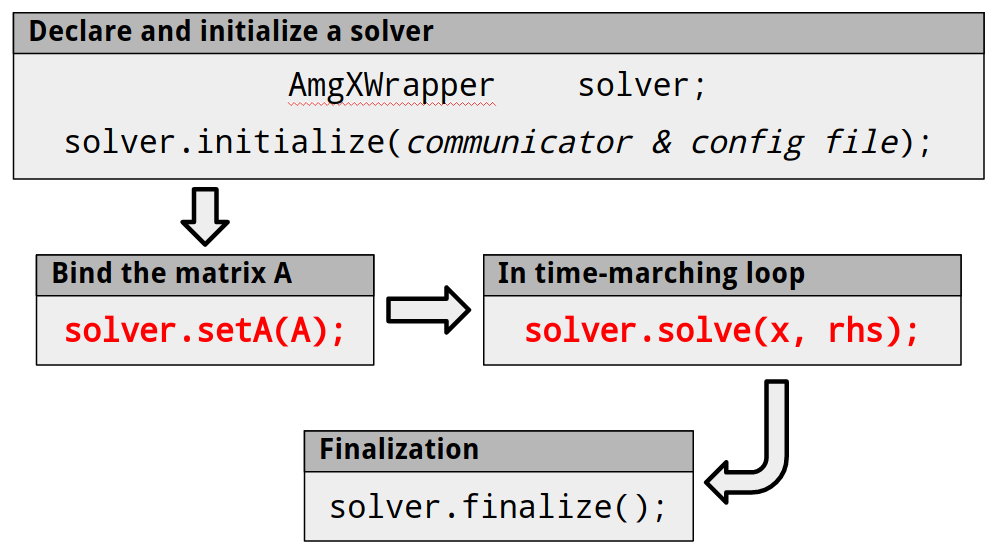
\includegraphics[width=0.6\linewidth]{amgxwrapper.png}
    \caption{Usage of AmgXWrapper in legacy PETSc applications}
    \label{fig:amgxwrapper}
\end{figure}

In addition to serve as a translation layer, AmgXWrapper also resolves an issue happens when CPUs and GPUs are both used in calculation.
It is common that HPC clusters have much more CPU cores than GPUs.
So CFD practitioners usually favor using all CPU cores and GPUs for computing.
However, most multi-GPU libraries were not developed for this use case.
Including AmgX, they expect users to use the same number for both MPI processes and GPUs.
AmgXWrapper provides matrix consolidation mechanism for use case when CPU cores and MPI processes are greater than available GPUs.
For example, most GPUs even nowadays do not have enough memory to host a whole 3D CFD problem.
So users may choose to use CPUs for solving forcing and velocity systems as they are not performance bottlenecks.
And they only use GPUs for pressure solvers to save GPU memory usage.
Therefore, it's natural for these users to use as many CPUs for forcing and velocity, so domain decomposition is done using the same number of MPI processes on CPUs.
When calling pressure solvers on GPUs, the number of subdomains do not match the number of GPUs, and this is when the matrix consolidation layer comes into play, as shown in figure \ref{fig:amgxwrapper-consolidation}.
Without the consolidation layer, several MPI processes would share one GPU, causing a resource competition.

\begin{figure}[H]
    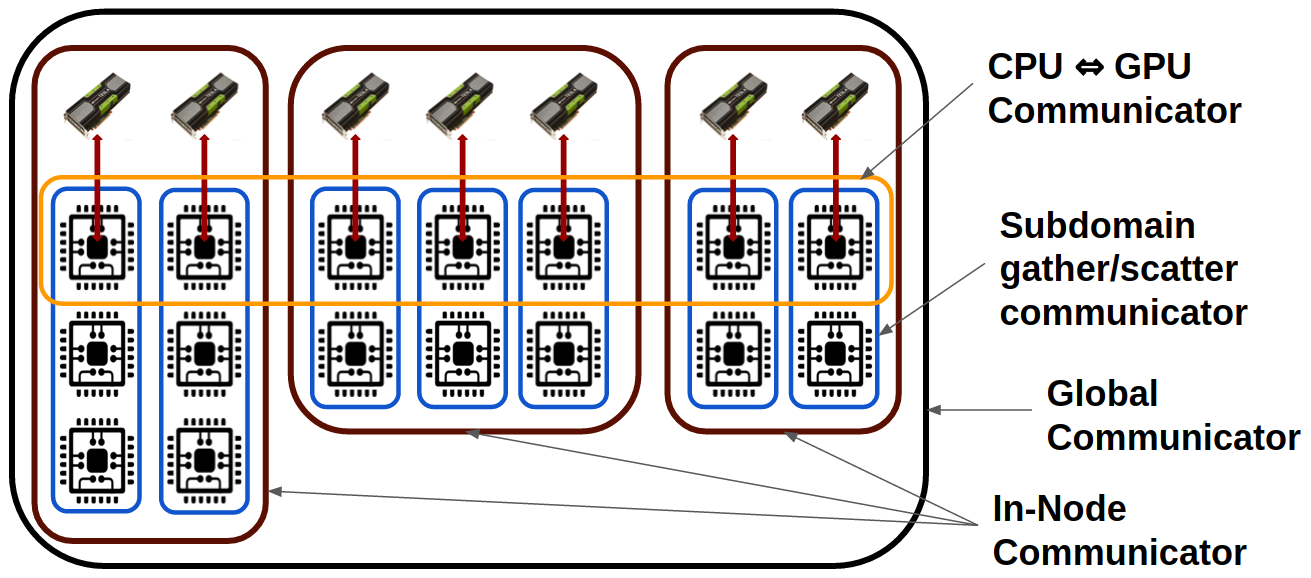
\includegraphics[width=0.6\linewidth]{amgxwrapper-consolidation.png}
    \caption{Graphic illustration of the consolidation layer in AmgXWrapper}
    \label{fig:amgxwrapper-consolidation}
\end{figure}

We will show the effect of the consolidation layer together with other performance benchmarks in section \ref{sec:petibm-perf}.
% vim:ft=tex

\section{Verification and Validation}\label{sec:petibm-vv}
%! TEX root = main.tex
This section shows cases for V\&V (verification and validation).
PetIBM is a baseline in PINN benchmarks, so its correctness must be confirmed.
These cases are: 2D and 3D Taylor\hyp{}Green vortex, 2D cylinder flows, 3D flow around a sphere, and 3D flow around an inclined flat plate.

\subsection*{Convergence test of 2D Taylor-Green vortex at $Re=100$}

The Taylor-Green vortex (TGV) represents a family of flows with a specific form of analytical initial flow conditions in 2D and 3D.
Specifically, 2D TGV problems with periodic boundary conditions have closed-form analytical solutions; hence, they usually serve as standard verification cases for CFD solvers. 
Here we used the following 2D Taylor-Green vortex to examine the order of convergence:
\begin{equation}\label{eq:tgv}
    \left\{
        \begin{aligned}
            u(x, y, t) &= V_0\cos(\frac{x}{L})\sin(\frac{y}{L})\exp(-2\frac{\nu}{L^2}t) \\
            v(x, y, t) &= - V_0 \sin(\frac{x}{L})\cos(\frac{y}{L})\exp(-2\frac{\nu}{L^2}t) \\
            p(x, y, t) &= -\frac{\rho}{4}V_0^2\left(cos(\frac{2x}{L}) + cos(\frac{2y}{L})\right)\exp(-4\frac{\nu}{L^2}t)
        \end{aligned}
    \right.
\end{equation}
$V_0$ represents the peak (and lowest) velocity at $t=0$;
$L$ is a scaling factor in the spatial domain;
$\nu$ and $\rho$ are kinematic viscosity and density, respectively.
$u$ and $v$ denote the velocity components in the $x$ and $y$ directions.
$p$ is the pressure.
The periodic boundary conditions are applied to $x=-L\pi$, $x=L\pi$, $y=-L\pi$, and $y=L\pi$.
As shown in the analytical solutions, the flow patterns do not change spatially, and only the amplitudes decay exponentially in time.

We used the following parameters for all our computational experiments: $V_0=L=\rho=1.0$ and $\nu=0.01$.
These parameters correspond to a Reynolds number of $Re=100$.

As the TGV problem only has periodic boundary conditions, there is no boundary discretization error in PetIBM that will taint the overall spatial convergence.
A 2nd-order grid convergence in space should therefore be expected.
The time marching schemes are Adams-Bashforth for the convection and Crank-Nicolson for the diffusion, so a 2nd-order convergence in time should also be observed.
Overall, the spatial-temporal convergence should be the 2nd-order.
Hence, we conducted a convergence test on spatial-temporal space for  convenience and simplicity.
The $L_2$ spatial-temporal error in this work is defined as:
\begin{equation}\label{eq:spt-err-def}
    \begin{aligned}
    L_{2,sp-t} \equiv &\sqrt{
        \frac{1}{L_x L_y T}
        \int\limits_{x} \int\limits_{y} \int\limits_{t} \lVert f - f_{ref} \rVert^2 \diff x \diff y \diff t
    } \\
    = &
    \sqrt{\frac{1}{N_x N_y N_t}\sum\limits_{i=1}^{N_x}\sum\limits_{j=1}^{N_y}\sum\limits_{k=1}^{N_t}\left(f^{(i, j, k)} - f_{ref}^{(i, j, l)}\right)^2}
    \end{aligned}
\end{equation}
$N_x$, $N_y$, and $N_t$ represent the number of cells on the $x$, $y$, and $t$ axis.
$f$ is the flow quantity of our interest, and $f_{ref}$ is the corresponding analytical solution.
The superscript $(i, j, k)$ denotes the value at the $(i, j, k)$ point in the discretized spatial-temporal space.
The characteristic cell size in a spatial-temporal sense is simply $\sqrt[3]{\frac{1}{N_x N_y N_t}}$, meaning the characteristic number of cells is $\sqrt[3]{N_x N_y N_t}$.

We ran simulations with $2^{n} \times 2^{n}$ cells for $i=4$, $5$, $\dots$, $10$.
The simulations ran from $t=0$ up to $t=100$, and we output the transient results every $2$ seconds of $t$.
The time step size $\Delta t$ did not follow a fixed refinement ratio.
Rather, it was refined based on the maximum allowed CFL number and whether it was a factor of $2$ (to output transient results).
The corresponding time step sizes were $\Delta t = 1.25\times 10^{-1}, 8\times 10^{-2}, 4\times 10^{-2}, 2\times 10^{-2}, 1\times 10^{-2}, 5\times 10^{-3}, 1.25\times 10^{-3}$.
The linear solvers for both velocity and pressure systems were solved with BiCGSTAB (biconjugate gradient stabilized method).
The velocity and pressure systems used a block Jacobi preconditioner and an algebraic multigrid preconditioner from AmgX.
At each time step, both solvers stopped when preconditioned residual reached $1\times 10^{-14}$.
The hardware contains 5 physical cores of Intel E5-2698 v4 and 1 V100 GPU.

Figure \ref{fig:petibm-tgv2d-re100-conv} shows the grid convergence results.
\begin{figure}[hbt!]
    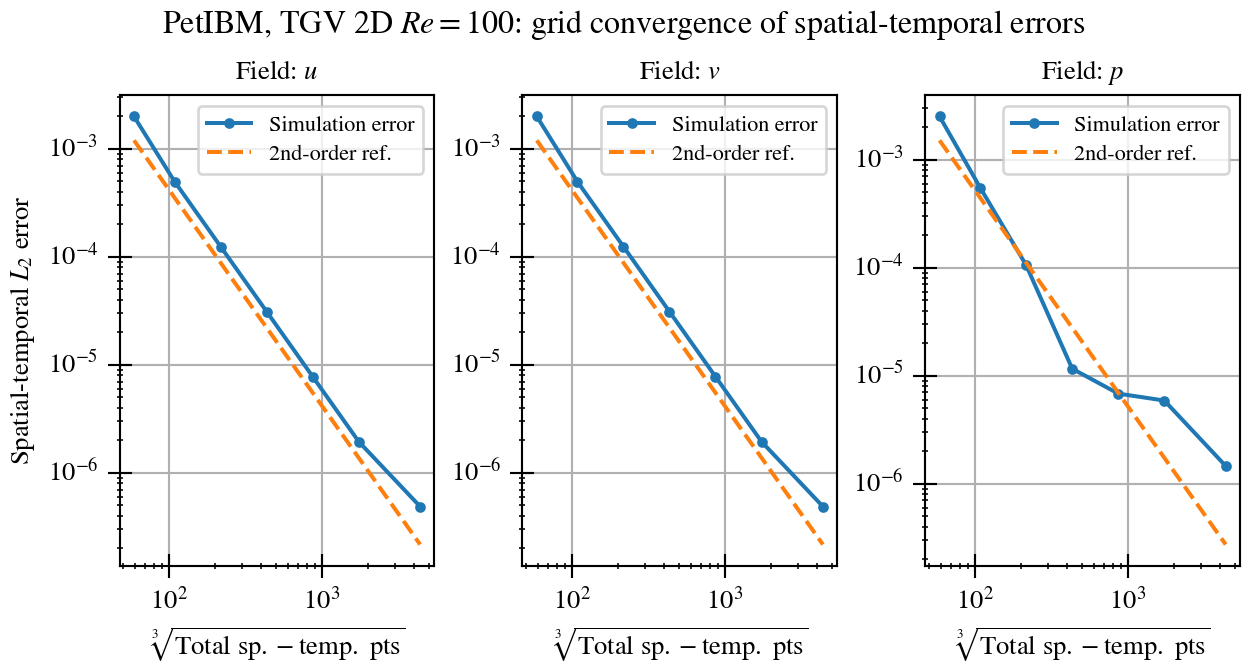
\includegraphics[width=0.75\linewidth]{tgv-2d-re100/petibm-tgv-2d-re100-convergence}
    \caption{PetIBM, 2D TGV, $Re=100$: spatial-temporal grid convergence}
    \label{fig:petibm-tgv2d-re100-conv}
\end{figure}
Both $u$ and $v$ velocities follow an expected 2nd-order convergence before machine roundoff errors become non-trivial at the $1024 \times 1024$ grid.
However, the pressure field does not follow such a nice convergence pattern.
After examining the log files, we determined that the cause was that AmgX did not solve the pressure systems to the tolerance we defined.
AmgX has a hard-coded stop mechanism when relative residuals (relative to the residual before the 1st iteration in a Krylov solver) reach the machine precision.
So while we configured the tolerance to be $1\times 10^{-14}$, the final preconditioned residuals of the pressure systems did not match this value.
On the other hand, the velocity systems were solved to the requested tolerance.

As we determined that the cause of the deviated convergence in pressure was irrelevant to the numerical method implementation, we concluded that the 2D TGV verification was successful.

\subsection*{Verification of 3D Taylor-Green vortex at $Re=1600$}

3D TGV problems have closed-form initial conditions but do not have closed-form analytical solutions.
These 3D TGV problems differ from 2D TGV cases due to the transition to turbulence.
Hence, it serves as a standard benchmark for turbulence simulations.
For example, see the campaign described in reference \cite{noauthor_1st_2012}. 
We compared the results to other published simulation data \cite{debonis_solutions_2013} in this verification.

The initial condition used was
\begin{equation}\label{eq:tgv3d-ic}
    \left\{
    \begin{aligned}
        u &=V_{0} \sin \left(\frac{x}{L}\right) \cos \left(\frac{y}{L}\right) \cos \left(\frac{z}{L}\right) \\
        v &=-V_{0} \cos \left(\frac{x}{L}\right) \sin \left(\frac{y}{L}\right) \cos \left(\frac{z}{L}\right) \\
        w &=0 \\
        p &=\frac{\rho V_{0}^{2}}{16}\left(\cos \left(\frac{2 x}{L}\right)+\cos \left(\frac{2 y}{L}\right)\right)\left(\cos \left(\frac{2 z}{L}\right)+2\right)
    \end{aligned}
    \right.
\end{equation}
We used $\rho = V_0 = L = 1$ and $\nu=0.000625$, corresponding to $Re \equiv \frac{V_0 L}{\nu} = 1600$.
The computational domain is $-L\pi$ to $L\pi$ for all three directions.

Due to the hardware required for high-resolution 3D DNS simulations for turbulent flow, we did not run the simulation with the spatial resolution suggested by reference \cite{noauthor_1st_2012}.
Our spatial resolution was $N_x=N_y=N_z=256$ with $\Delta t=0.01$.
The simulation ran up to $t=20$.
The hardware used was 128 physical CPU cores of AMD EPYC 7742 and 4 A100 GPUs (the 80GB variant).
It required about 250GB of memory, and the run time was 37 minutes.

Figure \ref{fig:petibm-tgv3d-re1600-val} shows that the mean kinetic energy qualitatively matches the reference data in \cite{noauthor_1st_2012} and \cite{debonis_solutions_2013}.
\begin{figure}[hbt!]
    \centering
    \begin{subfigure}[b]{0.45\textwidth}
        \centering
        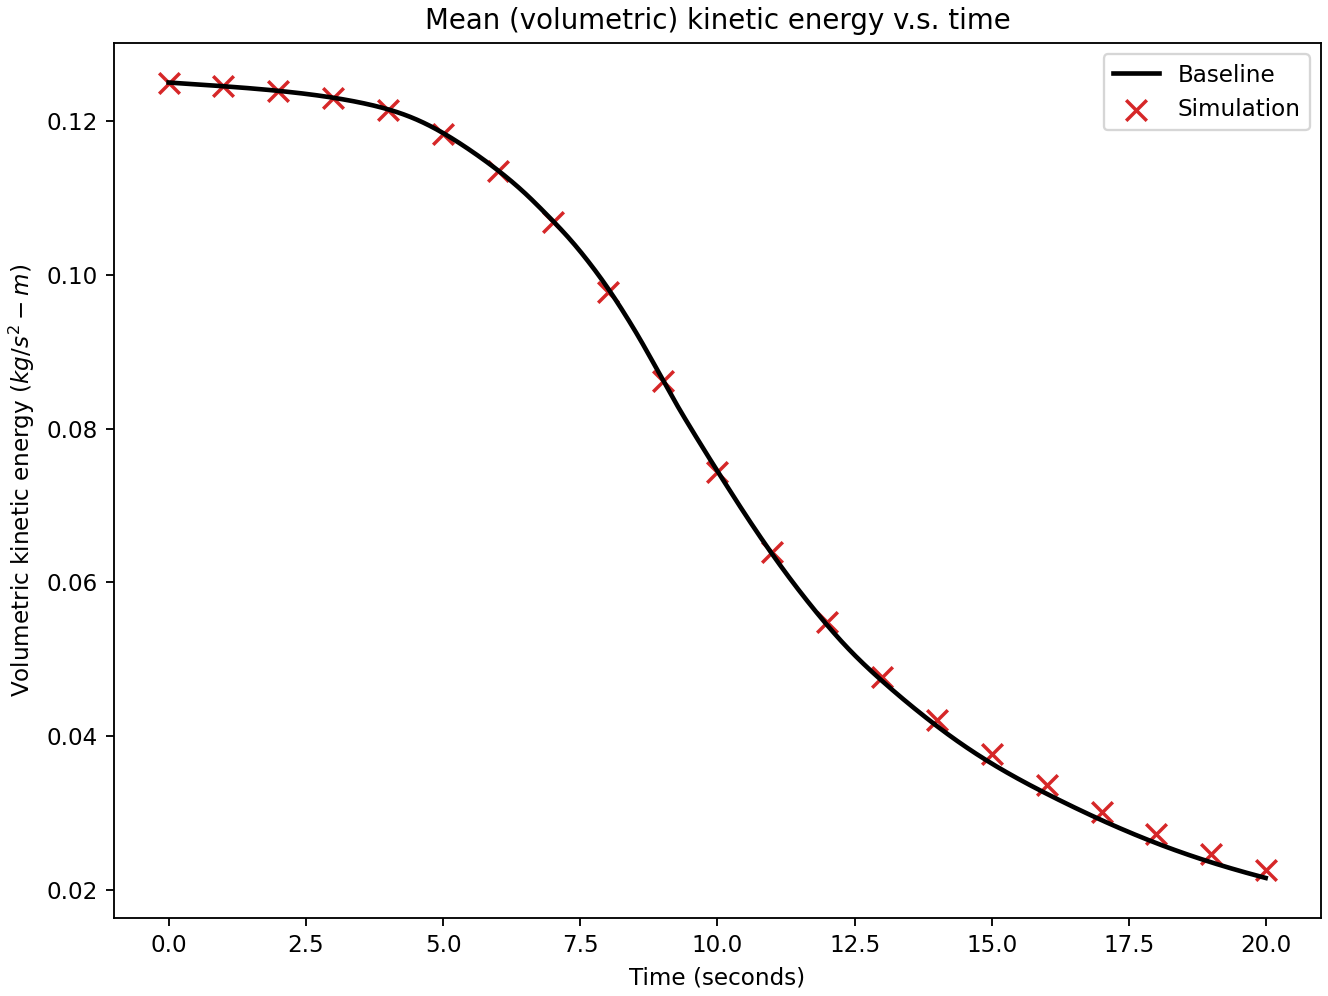
\includegraphics[width=\textwidth]{tgv-3d-re1600/mean-kinetic-energy}
        \caption{Mean kinetic energy}
        \label{fig:petibm-tgv3d-re1600-mean-energy}
    \end{subfigure}
    \hfill
    \begin{subfigure}[b]{0.45\textwidth}
        \centering
        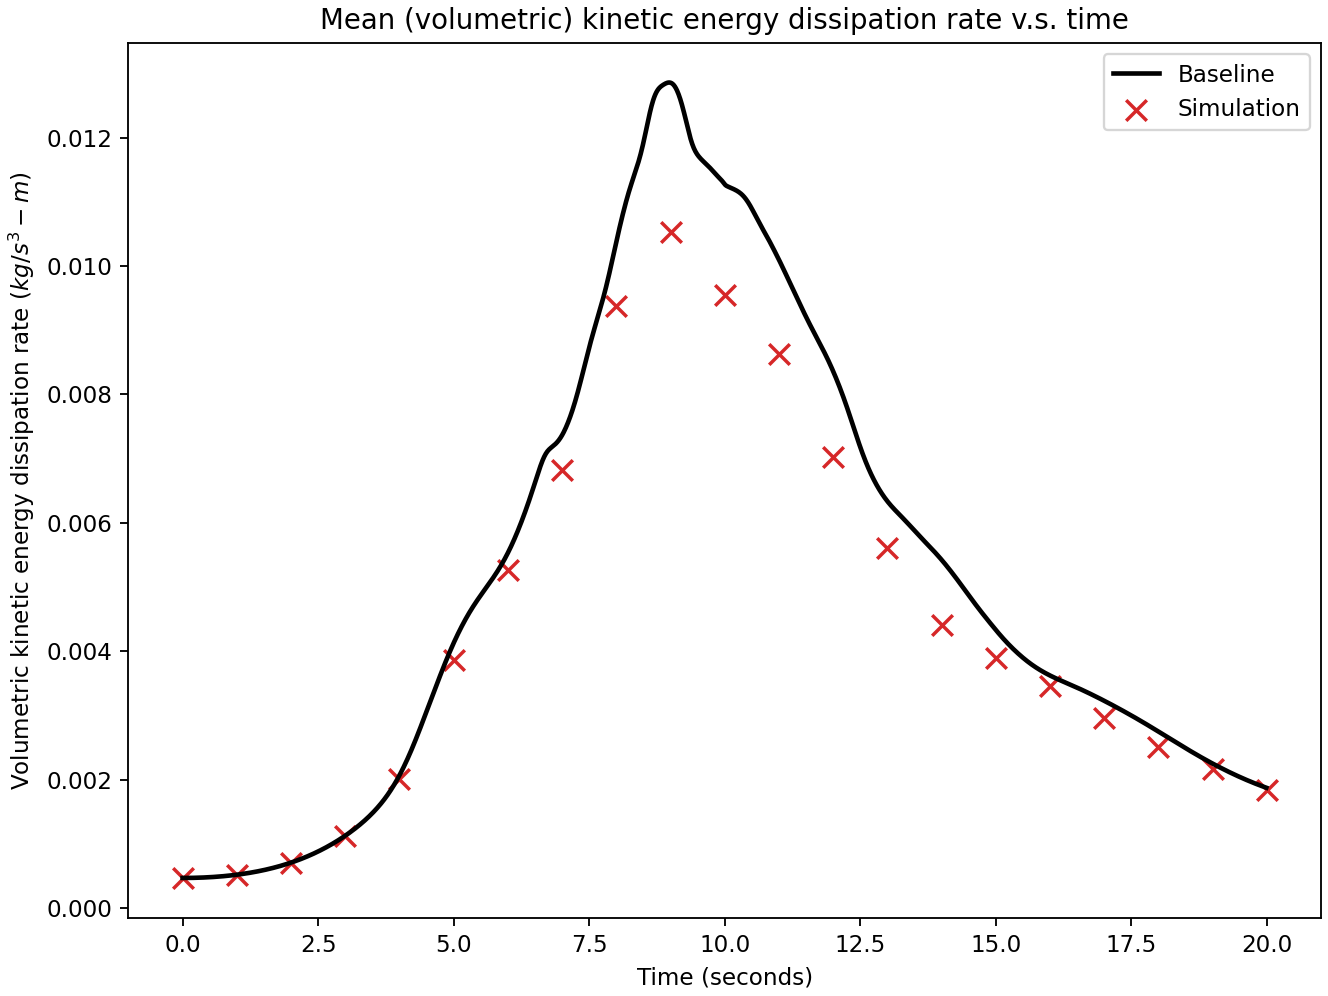
\includegraphics[width=\textwidth]{tgv-3d-re1600/mean-kinetic-energy-dissipation-rate}
        \caption{Mean kinetic energy dissipation rate}
        \label{fig:petibm-tgv3d-re1600-mean-energy-dissp}
    \end{subfigure}
    \caption{PetIBM, 3D TGV, $Re=1600$: validations}
    \label{fig:petibm-tgv3d-re1600-val}
\end{figure}
However, a visible mismatch exists in the mean kinetic energy dissipation rate.
Besides lower spatial resolution, another likely source of error is in the post-processing rather than in the numerical method implementation.
We calculated the dissipation rate using enstrophy, which requires post-processing steps due to using a staggered grid.
First, we applied the curl operator to the velocity defined on the staggered grid, and the resulting vorticity was also distributed staggered.
Next, we applied the linear interpolation operator and collected values from staggered grid points to cell centers.
Finally, we integrated the cell-centered vorticity using a simple 1st-order numerical integration.
Hence, we suspect that the post-processing largely contributed to the energy dissipation rate error.

Even some results from the campaign of references \cite{noauthor_1st_2012} and \cite{debonis_solutions_2013} show this level of mismatch in the dissipation rate.
Therefore, we conclude the 3D TGV verification at this point.
We do not claim that PetIBM's results match the reference data.
Nevertheless, it does not show any concerning problems in the comparison, either.

\subsection*{Validation and verification of 2D Cylinder flows}

In this work, a total of three different 2D cylinder flows were simulated: $Re=40$, $Re=100$, and $Re=200$.
In Williamson's stability categorization \cite{williamson_vortex_1996}, they correspond to the stable, 2D instability, and 2D to 3D transitioning regimes.
The cases of $Re=40$ and $Re=200$ were used for benchmarking PINNs.
Their results and V\&V can be found in chapter \ref{chap:pinn-cases}.
In this section, we only verify and validate our numerical solutions with $Re=100$.

The computational domain was $[-15$, $35]$ $\times$ $[-25$, $25]$ with a spatial discretization of $510$ $\times$ $298$.
Gridlines were stretched so that the cell size around the cylinder is about $\Delta x = \Delta y \approx 0.01\bar{6}$.
The time step size was $\Delta t = 0.01$.
The freestream condition of $u_{\infty}=1$ and $v_{\infty}=0$ were applied to the inlet, top, and bottom boundaries, while the outlet was convective BC.
The no-slip BC was applied to the cylinder surface.
The IC was $u_0=1$.
The configurations of the linear solvers in the velocity and the pressure systems were the same to those described in 2D TGV cases.
In addition, this case has an extra forcing system (equation \eqref{eq:dibpm-order2-2}), and it was solved using LU decomposition on CPUs through distributed SuperLU.
The hardware used was a node with 6 cores of intel i7-5930K and 1 K40 GPU.
It took about 10 minutes to finish the simulation.

\begin{table}[hbt!]
    \singlespacing
    \begin{threeparttable}[b]
        \begin{tabular}{lcc}
            \toprule
            & $C_{pb}$ \\
            \midrule
            PetIBM & -0.732   \\
            Williamson \& Roshko (1990) \tnote{1} & -0.736 \\
            \bottomrule
        \end{tabular}%
        \begin{tablenotes}
            \footnotesize
            \item [1] Through \cite{williamson_vortex_1996}. The third digit after the decimal point is an estimation as the value was obtained from digitizing a figure.
        \end{tablenotes}
        \caption[
            PetIBM, 2D Cylinder, $Re=100$: back suction coefficient validation with experimental data%
        ]{%
            2D Cylinder, $Re=100$: back suction coefficient validation with experimental data%
        }%
        \label{table:cylinder-2d-re100-cpb}
    \end{threeparttable}
\end{table}%
\begin{table}[hbt!]
    \singlespacing
    \begin{threeparttable}[b]
        \begin{tabular}{lcc}
            \toprule
            & $C_D$ & $St$ \\
            \midrule
            PetIBM & 1.36 & 0.174  \\
            Kim et al. (2001) \cite{kim_immersed-boundary_2001} & 1.33 & 0.165 \\
            Calhoun (2002) \cite{Calhoun2002} & 1.35\pm 0.014 & 0.175 \\
            Russell \& Wang (2003) \cite{Russell2003} & 1.38 \pm 0.007 & 0.169 \\
            Choi et al. (2007) \cite{choi_immersed_2007} & 1.34 \pm 0.011 & 0.164 \\
            \bottomrule
        \end{tabular}%
        \caption[%
            PetIBM, 2D Cylinder, $Re=100$: verification of drag coefficients and Strouhal number%
        ]{%
            Verification of net drag coefficients ($C_D$) and Strouhal numbers ($St$) for 2D cylinder flow at $Re=100$.%
        }%
        \label{table:cylinder-2d-re100-comparison-cd}
    \end{threeparttable}
\end{table}%

\begin{figure}[hbt!]
    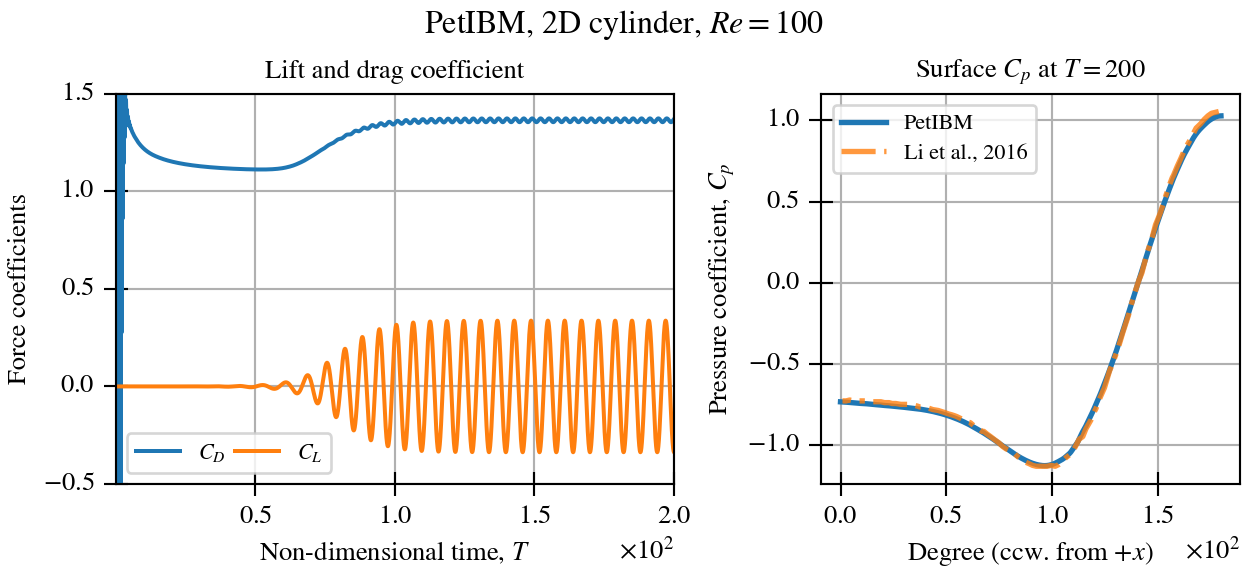
\includegraphics[width=0.95\linewidth]{cylinder-2d-re100/petibm-cylinder-2d-re100-val}
    \caption{PetIBM, 2D cylinder, $Re=100$: drag, lift, and pressure coefficients}
    \label{fig:petibm-cylinder-2d-re100-val}
\end{figure}

Table \ref{table:cylinder-2d-re100-cpb} shows the validation of the back suction coefficient, $C_{pb}$ (i.e., the surface pressure coefficient at the downstream end of the cylinder) against experimental data.
The drag coefficient and Strouhal number were verified with others' published numerical data and shown in table \ref{table:cylinder-2d-re100-comparison-cd}.
Figure \ref{fig:petibm-cylinder-2d-re100-val} shows the drag and lift coefficient with respect to time and the distribution of surface pressure coefficients.
The latter was verified against another published simulation result (see figure for the reference).

We determined that the V\&V for 2D cylinder flow at $Re=100$ was successful.

\subsection*{Validation of 3D flow around a sphere}

We validate the simulation results of 3D sphere flows at different Reynolds numbers.
These Reynolds numbers are $Re=50$, $100$, $150$, $200$, $250$, and $300$.
All cases used the same computational domain, $[-10$, $10]$ $\times$ $[-10$, $10]$ $\times$ $[-10$, $10]$, and the time step size $\Delta t=0.004$.
The corresponding grid sizes are $272$ $\times$ $82$ $\times$ $82$.
The BCs, ICs, and the linear solver configurations are the same as those in 2D cylinder flow at $Re=100$.

Figure \ref{fig:petibm-sphere3d-drag-val} shows the validation results against experimental data \cite{clift_bubbles_2013,roos_experimental_1971}.
\begin{figure}[hbt!]
    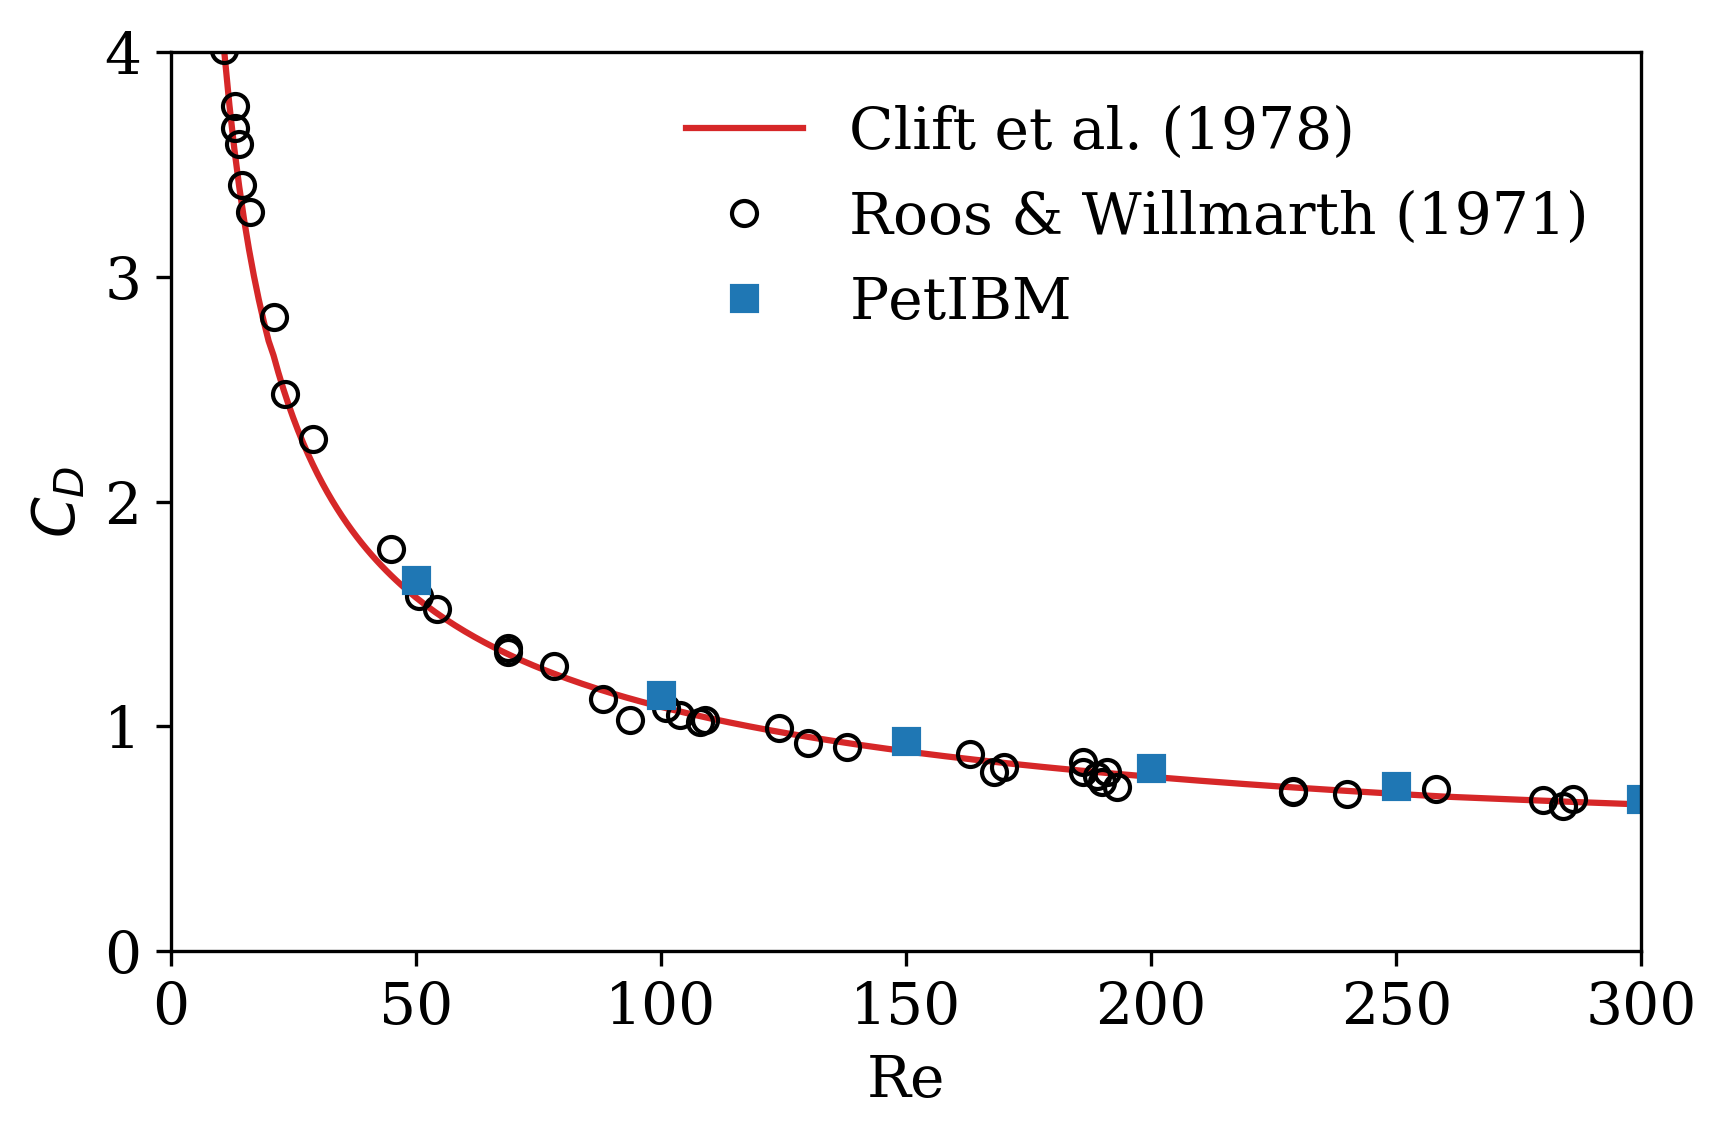
\includegraphics[width=0.6\linewidth]{sphere-3d/drag_coefficient}
    \caption[PetIBM, 3D sphere: drag coefficient validation]{
        PetIBM, 3D sphere: drag coefficient validation \cite{clift_bubbles_2013,roos_experimental_1971}
    }
    \label{fig:petibm-sphere3d-drag-val}
\end{figure}
We believe it is appropriate to call the validation of 3D sphere flow a success.

\subsection*{Validation of 3D flow around an inclined flat plate}

Lastly, we validate the solver using a 3D flow over an inclined flat plate at $Re=100$.
We tested with several AoA (angle of attack) and validated the results against the experimental data from reference \cite{taira_unsteadiness_2007}.
All cases had the same computational domain, $[-4$, $6.1]$ $\times$ $[-5$, $5]$ $\times$ $[-5$, $5]$, and the flat plate was located at $(0.1$, $1$, $1)$.
The spatial discretization is $192 \times 56 \times 86$, and the time step $\Delta t$ is $0.01$.
The BCs, ICs, and the linear solver configurations are the same as those in 2D cylinder flow at $Re=100$.

\begin{figure}[hbt!]
    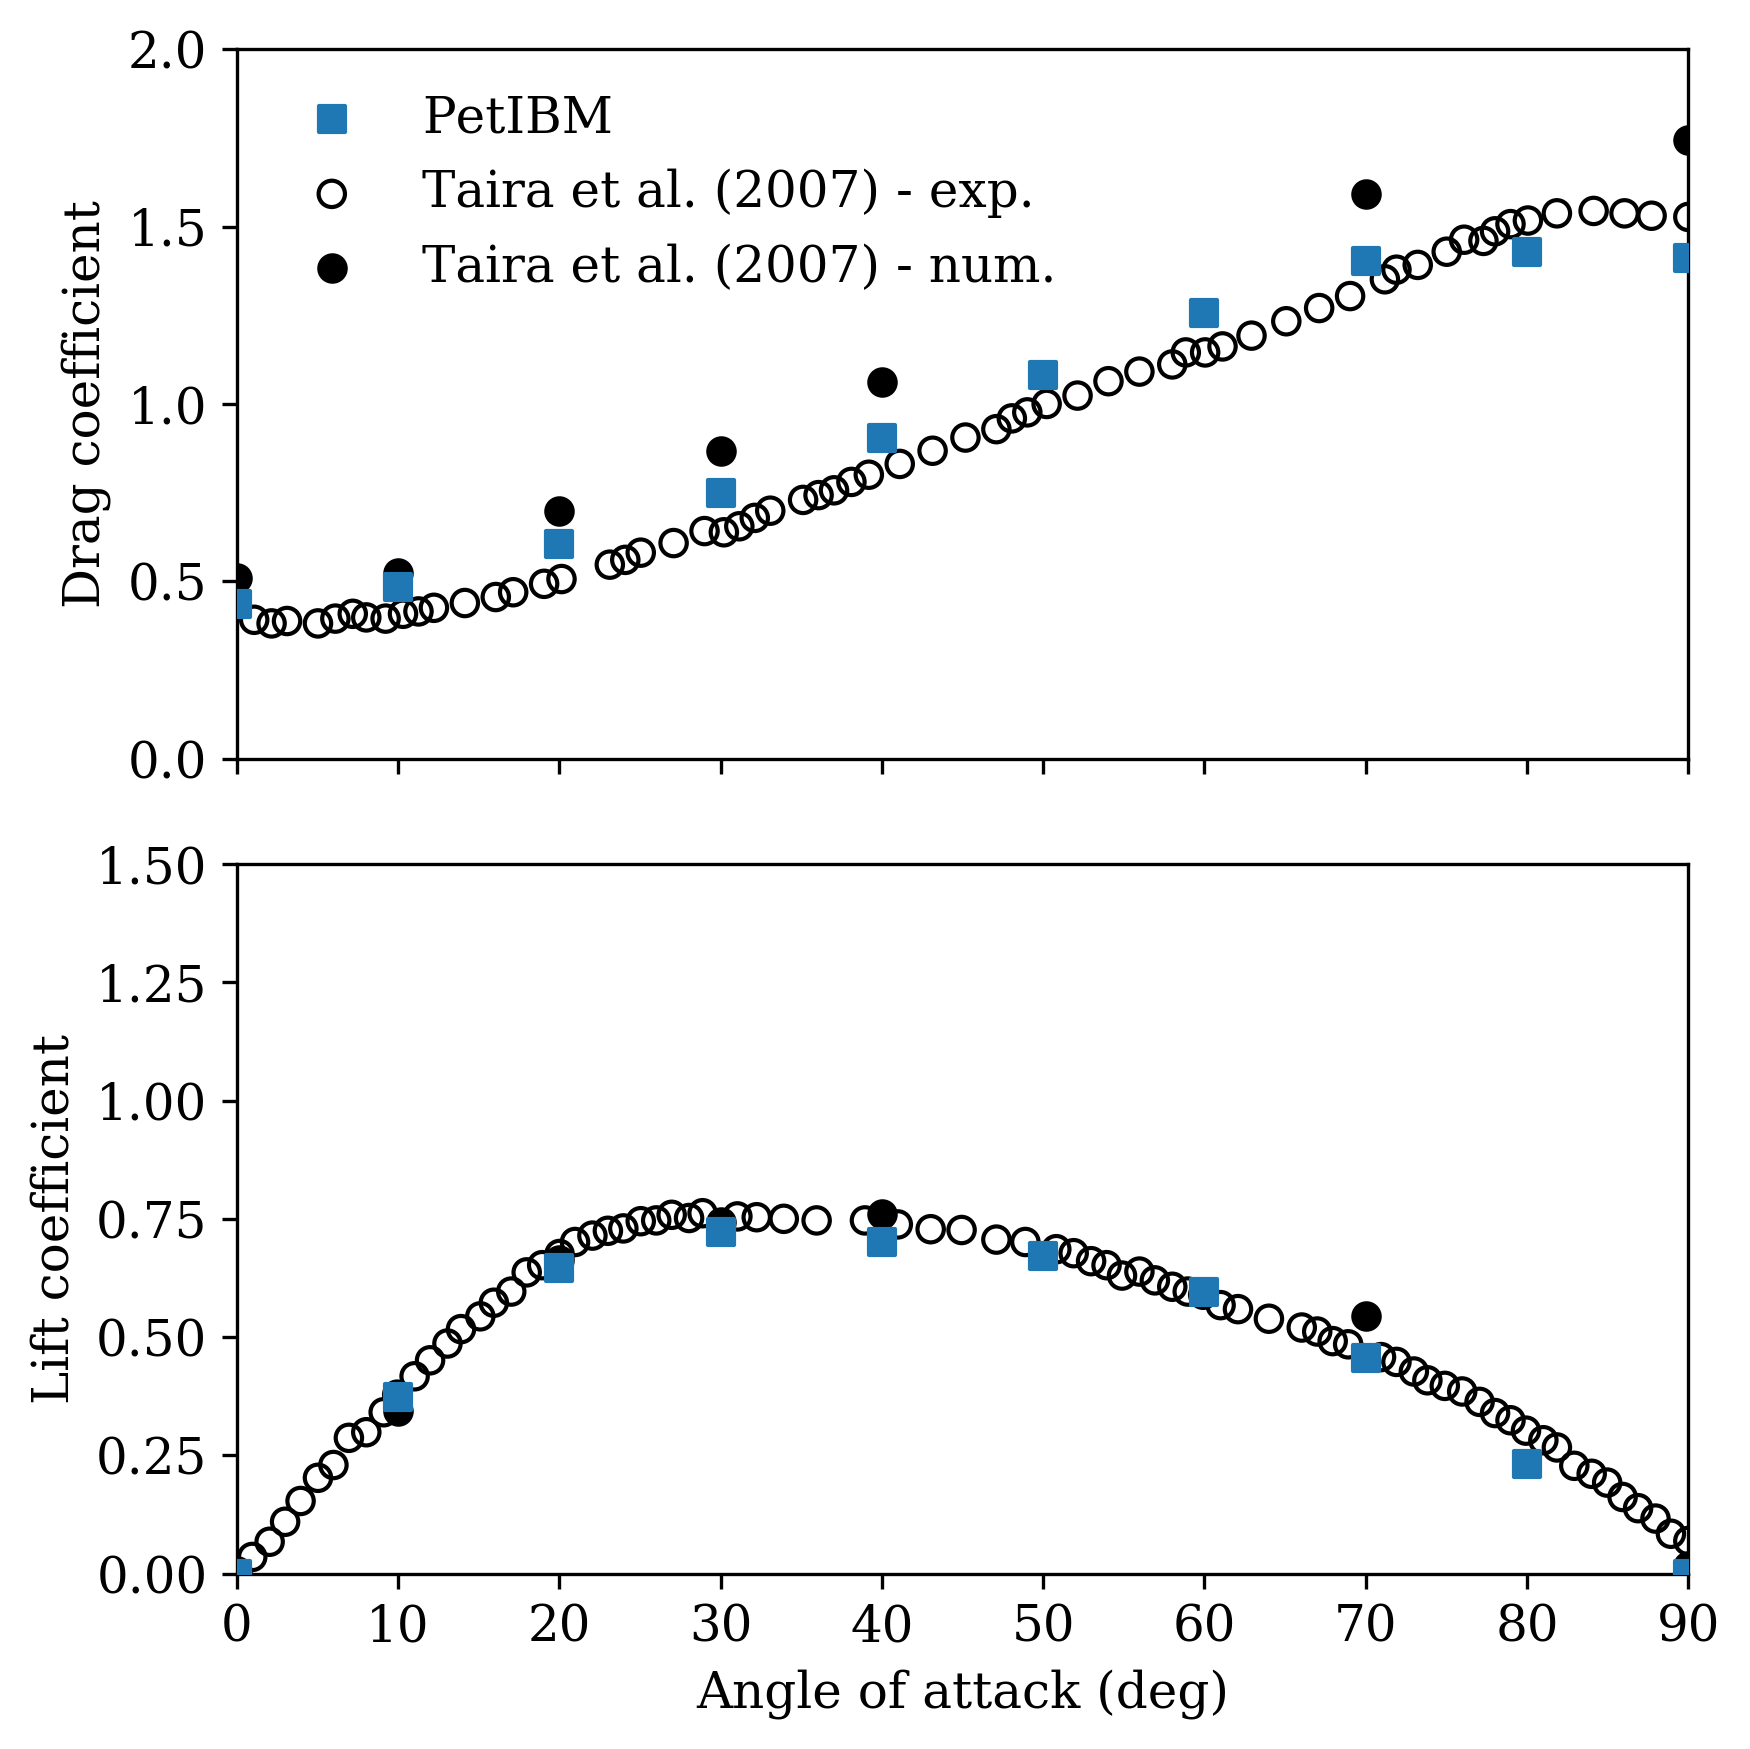
\includegraphics[width=0.6\linewidth]{plate-3d-re100/force_coefficients}
    \caption{PetIBM, 3D plate: drag and lift coefficient validation}
    \label{fig:petibm-plate3d-drag-lift-val}
\end{figure}
Figure \ref{fig:petibm-plate3d-drag-lift-val} shows that the experimental data matches our numerical simulation well.

% vim:ft=tex


\section{Performance Benchmarks}\label{sec:petibm-perf}
%! TEX root = main.tex

We first examined the performance of AmgXWrapper.
Figure \ref{fig:amgxwrapper-cons-1M} and \ref{fig:amgxwrapper-cons-15M} show the run time of solving Possion problems.
The former solves a smaller problem with $1$ million unknowns, and the latter has $15$ millions unknowns.
In each figure, on the left we have the performance before applying the consolidation mechanism in AmgXWrapper.
And on the right we show how the consolidation helps the performance.
The tests were done with NVIDIA V100 GPUs.

\begin{figure}[H]%
    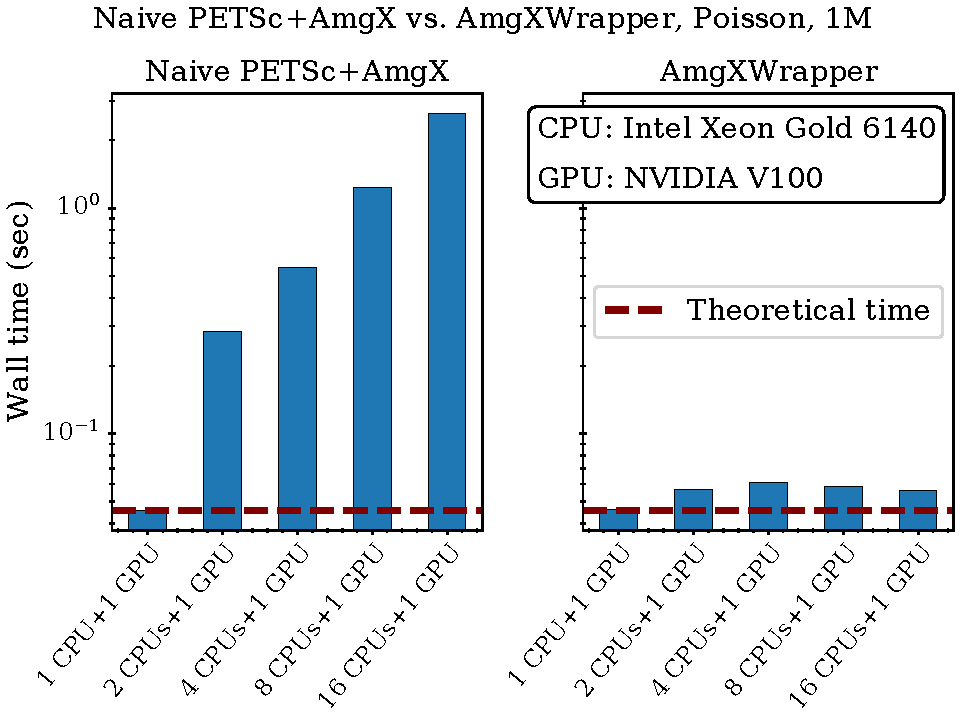
\includegraphics[width=0.6\linewidth]{amgxwrapper-consolidation-tests-poisson-1M}%
    \caption{AmgXWrapper benchmark: 3D Poisson problem w/ 1M unknowns and using 1 V100 GPU.}\label{fig:amgxwrapper-cons-1M}%
\end{figure}

\begin{figure}[H]%
    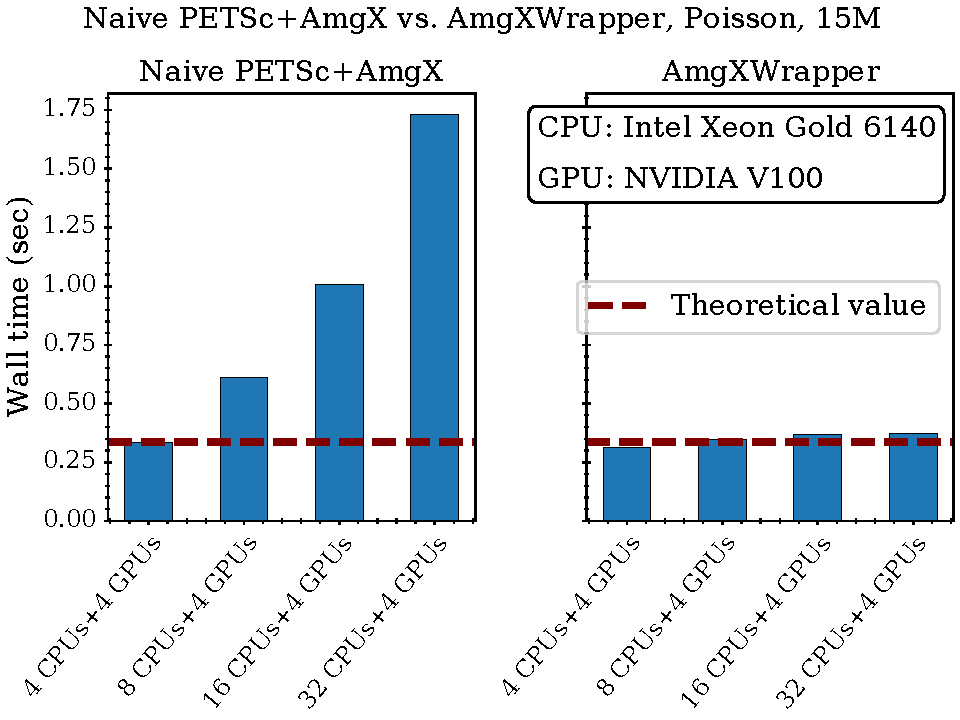
\includegraphics[width=0.6\linewidth]{amgxwrapper-consolidation-tests-poisson-15M}%
    \caption{AmgXWrapper benchmark: 3D Poisson problem w/ 15M unknowns and using 4 V100 GPUs.}\label{fig:amgxwrapper-cons-15M}%
\end{figure}

Bars in the figures represent the results of using different numbers of CPUs plus a fixed number of GPUs.
The smaller Poisson problem was solved with one GPU, while the larger problem was solved with 4 GPUs.
Using more CPUs speeds up the pre-processing stage, such as matrix creation because it means more subdomains and fewer unknowns per subdomain.
However, the run times of the solving stage should not be affected by the number of CPUs because the solver resides on GPUs completely, and we have a fixed number of GPUs.

Results in \ref{fig:amgxwrapper-cons-1M} and \ref{fig:amgxwrapper-cons-15M} show that this statement is not true for the plots on the left, that is, without consolidation. 
As more CPUs are used, run times grows linearly.
V100 was still the mainstream GPUs used on HPC clusters at the time of writing.
Yet the results show it was not designed for handling multiple tasks and does not handle well with resource competition.

The consolidation in the translation layer helps resolve the issue.
This mechanism consolidate and rearrange subdomains' matrices.
Rearranging is necessary as the performances of multigrid preconditioners may rely on the structures of submatrices on each GPU.
Plots on the right show that run times were close to a constant time regardless of how many CPUs were used.

The time used for consolidation was included in the solving stage shown in these two figures.
The smaller Poisson problem shows an overhead due to the consolidation.
However, for the larger problem, the overhead was not obvious as consolidation is a relative cheap operation compared to the actual solving. 

Next, in figure \ref{fig:amgxwrapper-speedups-15M} and \ref{fig:amgxwrapper-speedups-33M}, we show the speedups of GPU solvers versus CPU solvers on Poisson problems.
The former has $15$ millions of unknowns, while the latter has $33$ millions.
The plots also contains a visualization of the strong scaling.
The CPU tests used the conjugate-gradient (CG) solver from PETSc with the BoomerAMG preconditioner from Hypre.
The GPU tests used the CG solver and the classical multigrid preconditioner from AmgX.
Theoretically, these two configurations are comparable because AmgX's classical multigrid preconditioner was a re-implementation on GPU of BoomerAMG. 

\begin{figure}[H]
    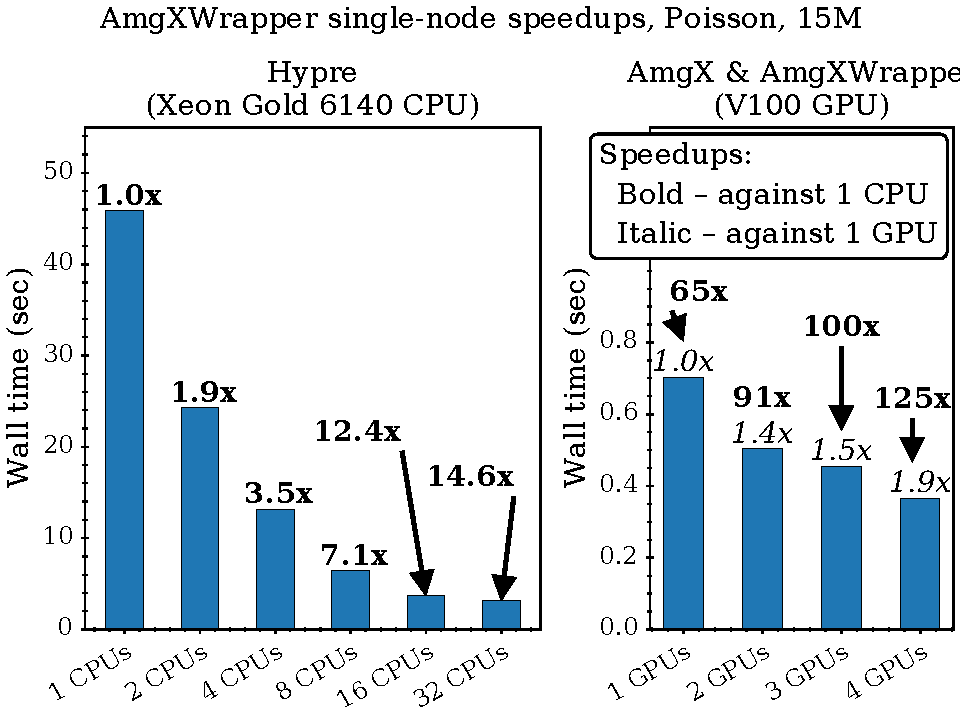
\includegraphics[width=0.6\linewidth]{amgxwrapper-proc-speedups-poisson-15M}
    \caption{Speedups of AmgXWrapper vs.\@ Hypre w/ 15M unknowns.}
    \label{fig:amgxwrapper-speedups-15M}
\end{figure}

\begin{figure}[H]
    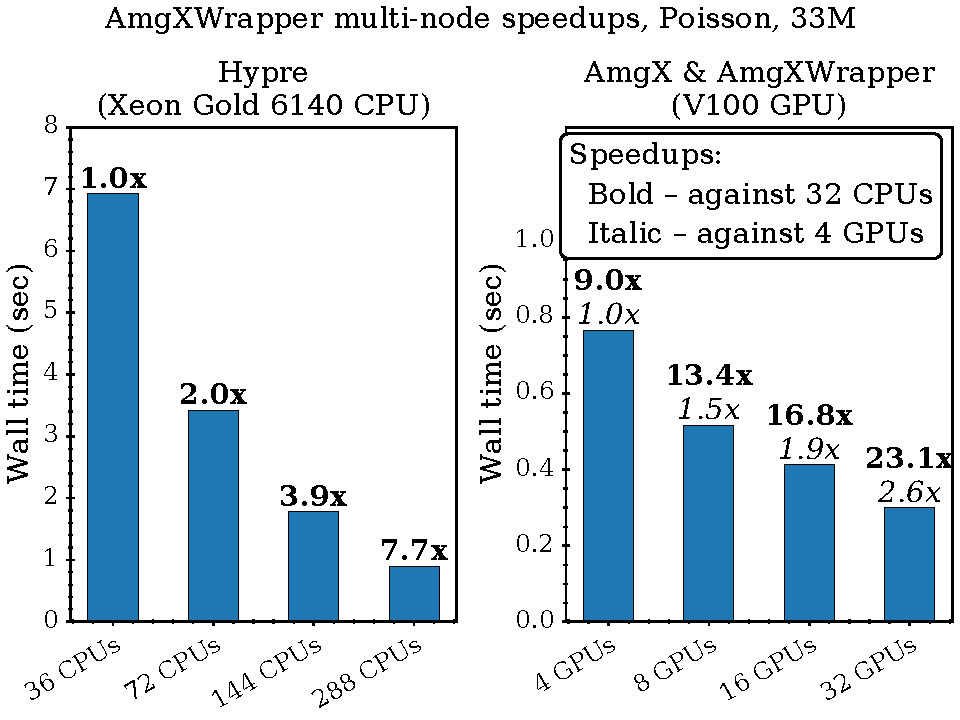
\includegraphics[width=0.6\linewidth]{amgxwrapper-node-speedups-poisson-33M}
    \caption{Speedups of AmgXWrapper vs.\@ Hypre w/ 33M unknowns.}
    \label{fig:amgxwrapper-speedups-33M}
\end{figure}

From the results, we observed a $65x$ speedup comparing 1 GPU to 1 CPU in the $15$-million problem and a $9x$ speedup comparing 4 GPUs to 36 CPUs in the $33$-million problem.
As a reference, at the time of writing, 4 V100 GPUs cost about $12$ thousand US dollars.
On the other hand, $36$ cores of CPUs consists of $2$ Xeon Gold 6140 chips, which cost around $2$ thousand US dollars\footnote{Xeon Gold 6140 was descontinued at the time or writing. The price we show here was the market value at the time, while the official suggested price for $2$ brand-new chips was around $4,800$ US dollars.}.
If we naively compare the results base on the monetary cost of the GPUs and CPUs, we would observe a speedup of about $1.5x$ (4 V100 GPUs versus 218 CPU cores).
However, as CPUs and GPUs work under different hardware configurations and setups, this monetary-based comparison is not fair in the real world.
For example, $6$ CPU chips may require $3$ complete computing nodes and an HPC cluster, while 4 V100 GPU can completely reside in one single workstation or even a personal desktop.
Under this argument, both the hardware cost and human labor cost (for maintenance) of CPUs will be much higher, and the speedups and cost saving from GPUs will be much more attractive.
Unfortunately, we were not able to get the cost estimation of a $3$-node HPC cluster and hence were not able to continue on the monetary cost comparisons.
Nevertheless, we hope our arguments can provide an impression on the hardware costs as these costs are often ignored in literature of performance benchmarks.

In terms of strong scaling, CPU solvers tended to show a better strong scaling.
For example, if we translate the speedup in the CPU results to strong scaling efficiencies for the smaller problem were about 95\%, 88\%, 88\%, 78\%, and 46\%, respectively.
And those of the larger problem were 100\%, 98\%, and 96\%.
In the GPU results, the strong scaling efficiencies of the small problem were 70\%, 50\%, and 48\%, while those of the larger problem were 75\%, 47\%, and 32\%.
From this viewpoint, CPU solvers give a better predictability on required resources and time-to-solutions. 

Finally, we were interested the actual performance gain in real flow simulation.
Figure \ref{fig:petibm-speedups-15M-small} and \ref{fig:petibm-speedups-15M-large} show the high-level performance profiling of PetIBM using a 3D flying-snake simulation \cite{krishnan_lift_2014,krishnan_cuibm_2017}.
The number of cells is $15$ millions, meaning there were about $45$ millions unknown in the velocity system and $15$ million unknowns in the pressure system.
The snake was discretized to $2,925$ Lagrangian points, meaning the forcing system has $8,775$ unknowns.

\begin{figure}[H]
    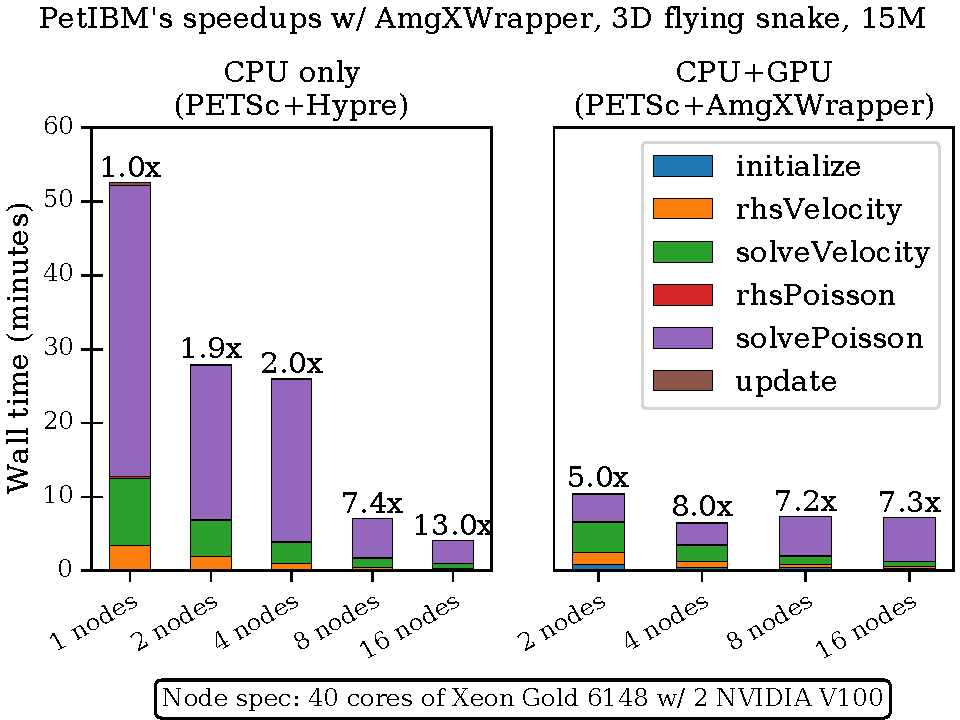
\includegraphics[width=0.6\linewidth]{petibm-speedups-scaling-small-gpu}
    \caption{Speedups of PetIBM: 2 V100 per node}
    \label{fig:petibm-speedups-15M-small}
\end{figure}

\begin{figure}[H]
    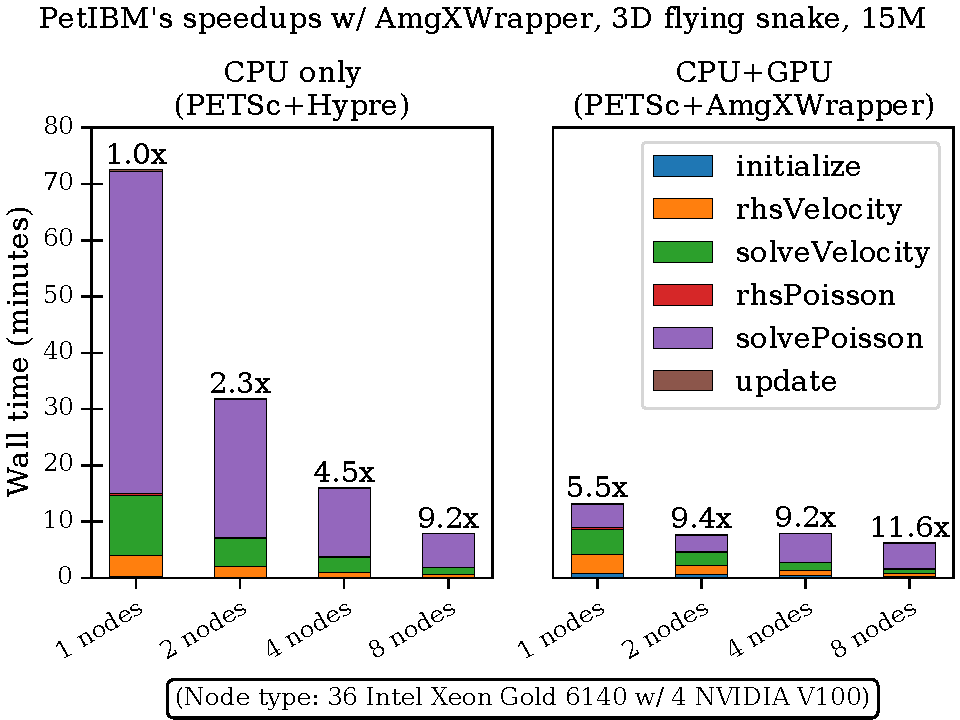
\includegraphics[width=0.6\linewidth]{petibm-speedups-scaling-large-gpu}
    \caption{Speedups of PetIBM: 4 V100 per node}
    \label{fig:petibm-speedups-15M-large}
\end{figure}

In CPU-only simulations, PetIBM solved velocity systems with the GAMG preconditioner and pressure systems with BoomerAMG preconditioner.
In CPU-GPU mixed simulations, the preconditioners for velocity and pressure systems are block-Jacobi and classical multigrid from AmgX, respectively.
The underlying Krylov solvers are the bi-conjugate gradient stabilized solver from either PETSc or AmgX.
The forcing systems in both types of simulations were solving by LU decomposition using distributed SuperLU.
This is the only part solved on CPU for the CPU-GPU mixed simulations.

The two figures show the performance speedups comparing pure-CPU and CPU-GPU-mixed simulations on two different clusters: one with 2 V100 per node, while the other one with 4 V100 per node.
We conducted the simulations on two different to ensure the results has generalizability.
The results from both clusters agree with each other.
We observed that one 4-GPU node or two 2-GPU nodes are equivalent roughly to 5 pure-CPU nodes.
The difference between the two clusters lies in that the 4-GPU nodes had less internode communication and hence had better performance and scalability.
% vim:ft=tex
% vim:ft=tex
